\chapter{Apêndices}

\section{Diagrama da Classe RF24}
  \begin{figure}[!htb]
    \centering
    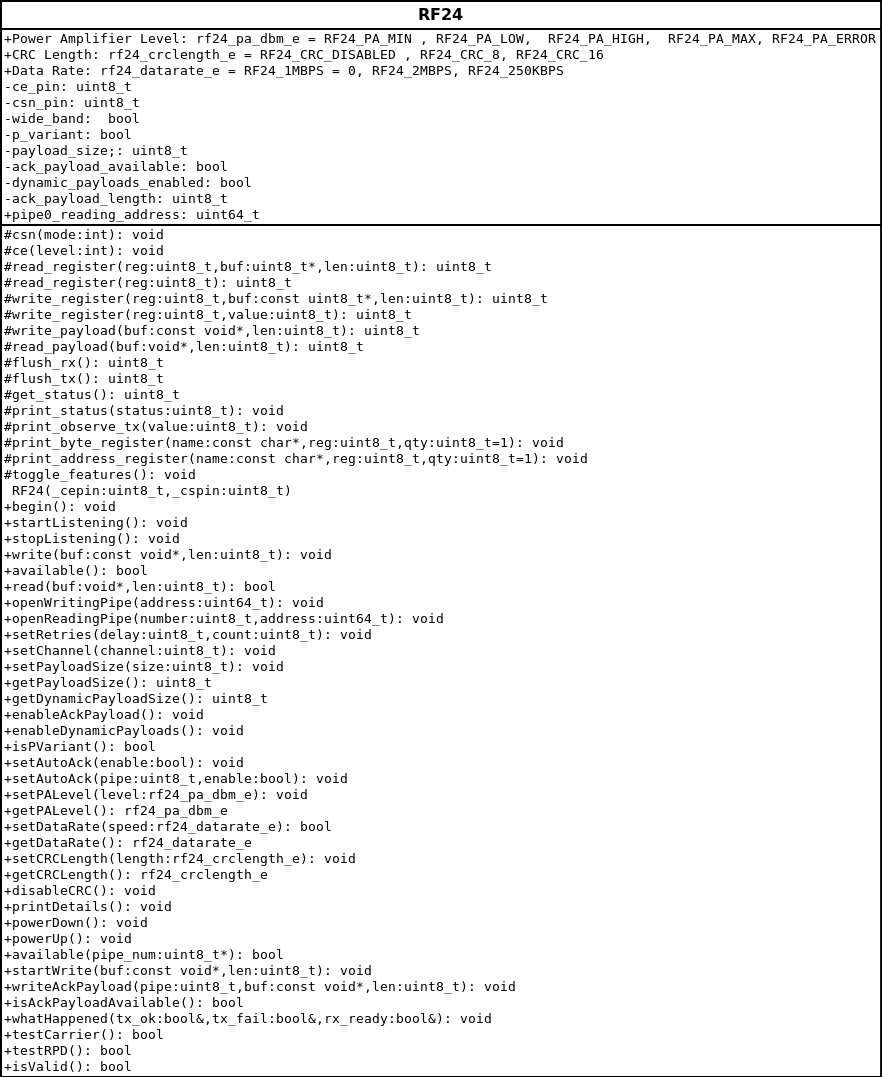
\includegraphics[width=\linewidth]{../../Imagens/RF24_class.png}
    \caption{Diagrama da Classe RF24} %% TODO certificar se realmente é uma WBS!!!
    \label{RF24_ClassDiag}
  \end{figure}

\section{Estrutura Analítica do Projeto}
  \begin{figure}[!htb] %% TODO certificar se realmente é uma WBS!!!
    \centering
    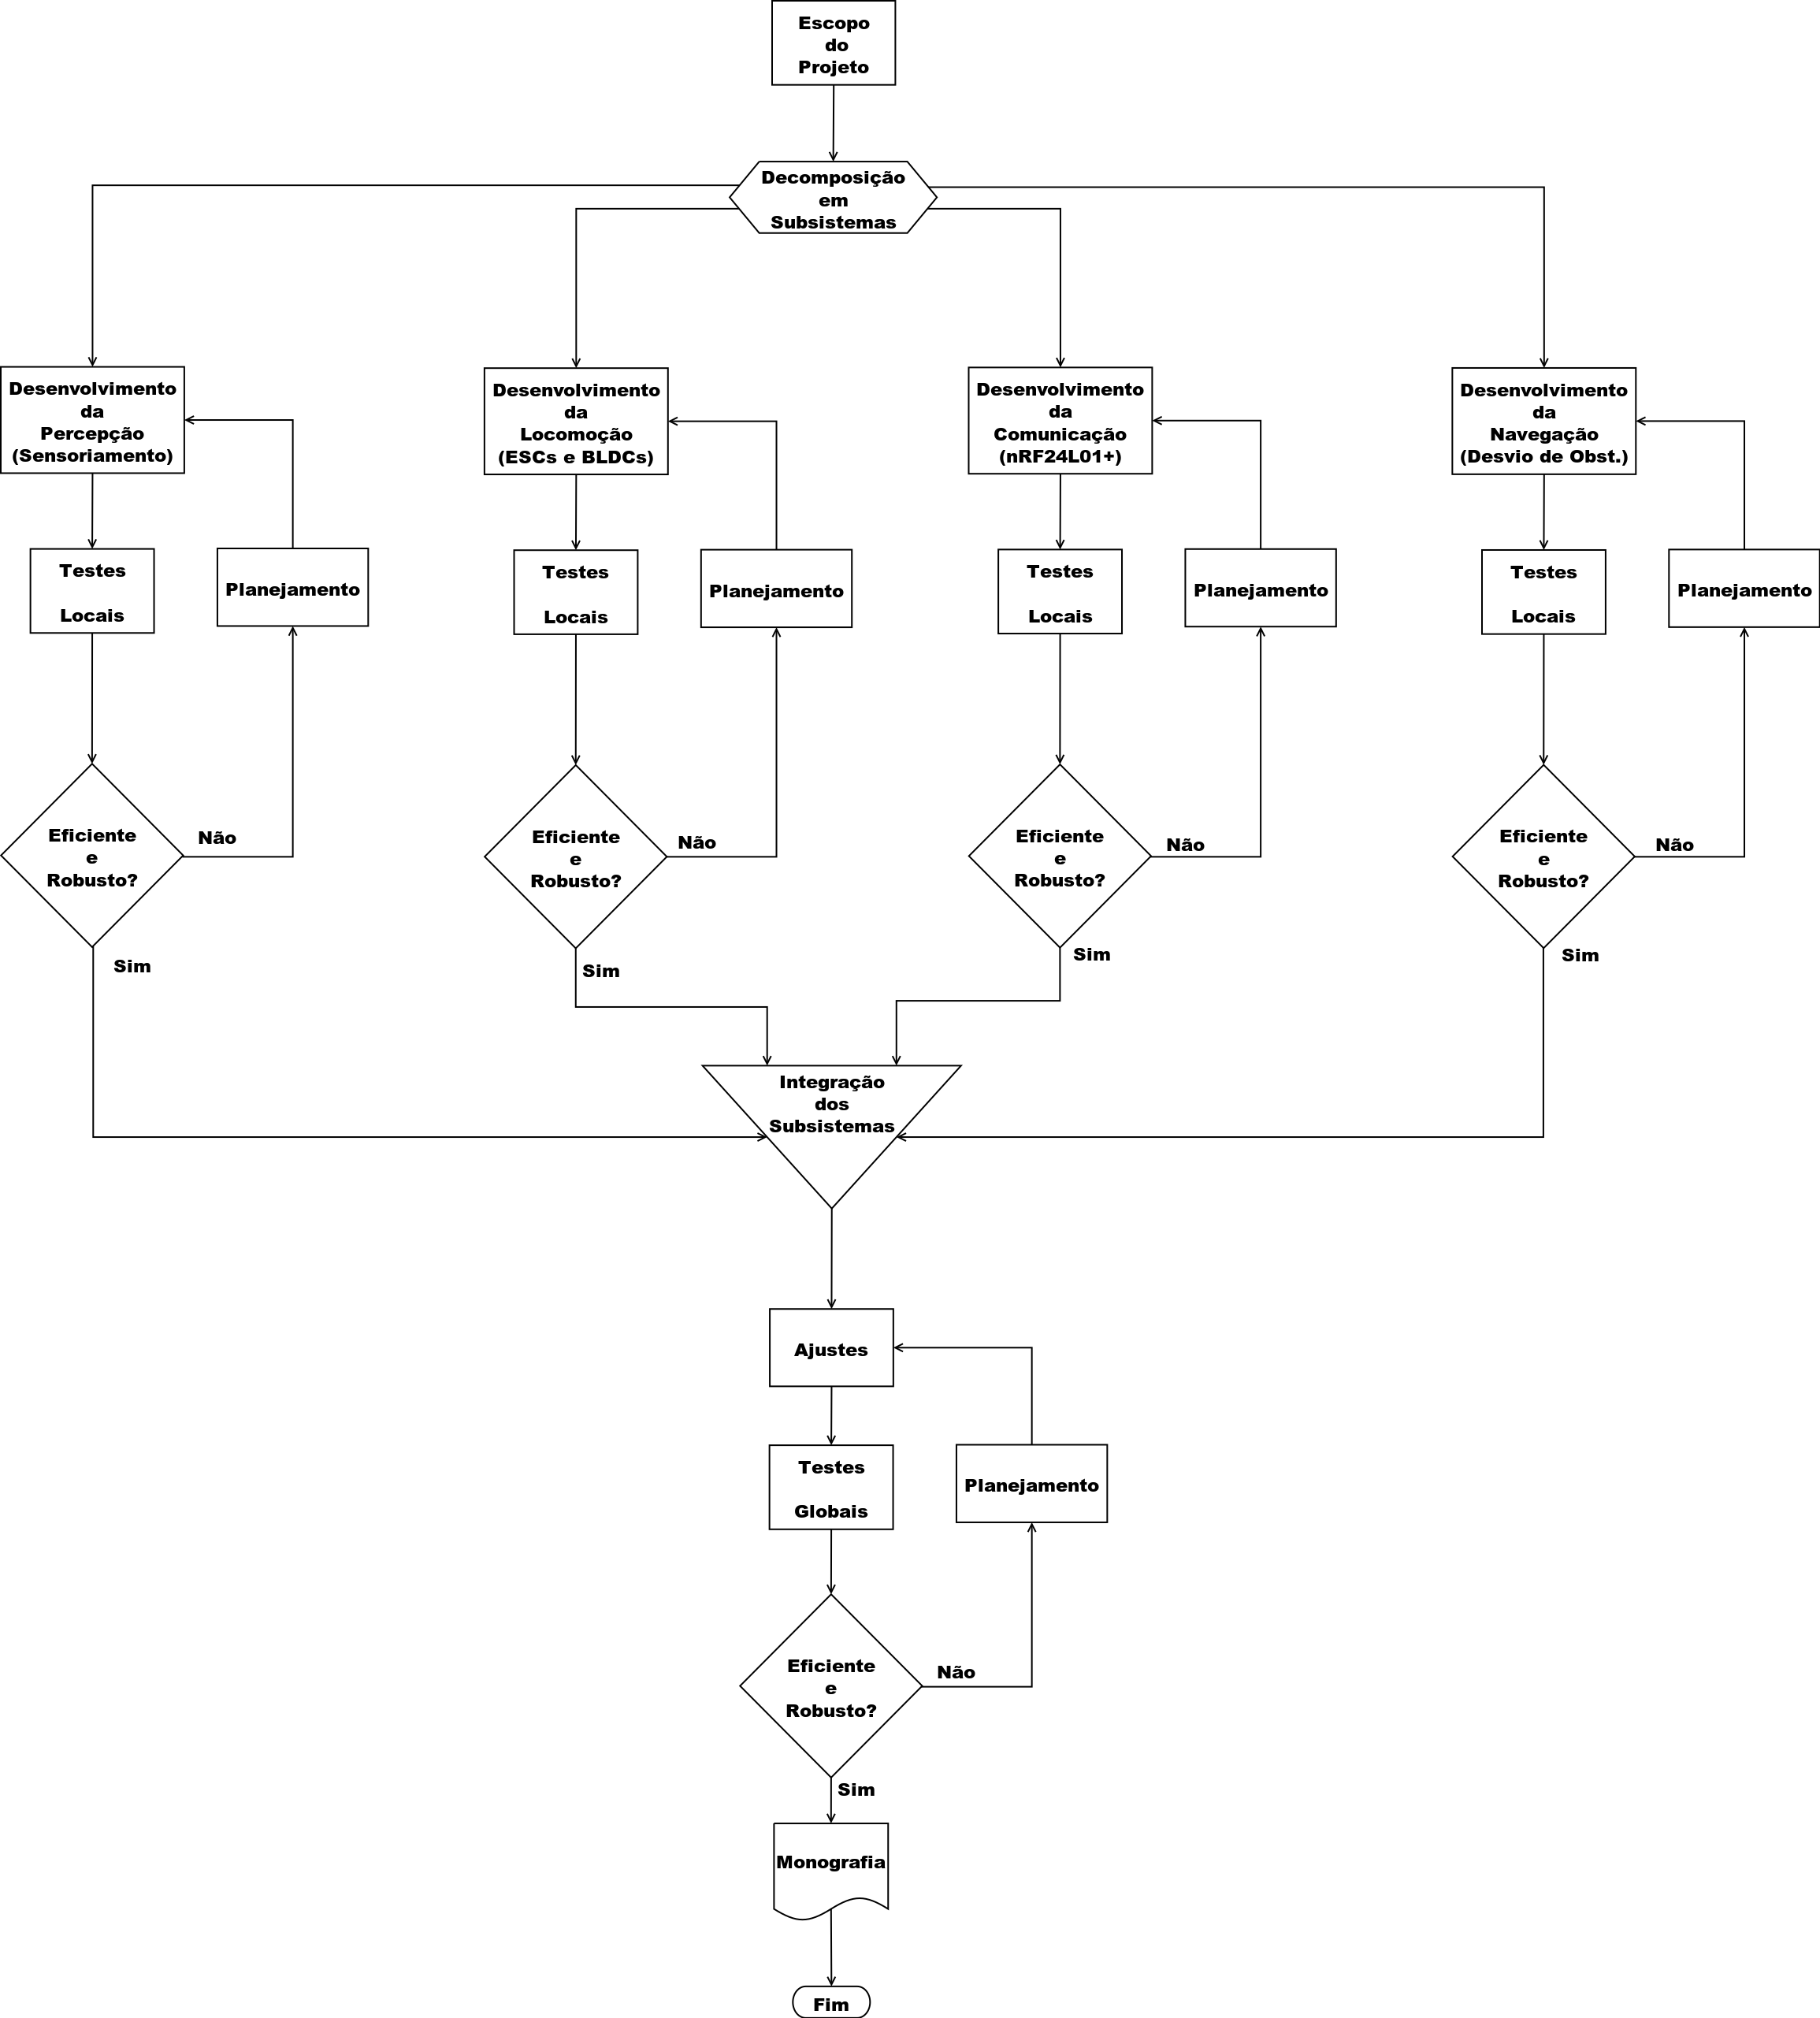
\includegraphics[width=\linewidth]{../../Imagens/WBS.png}
    \caption{Estrutura Analítica do Projeto} %% TODO certificar se realmente é uma WBS!!!
    \label{WBS}
  \end{figure}
  
\section{Esquemático do Robô}
  \begin{figure}[!htb]
    \centering
    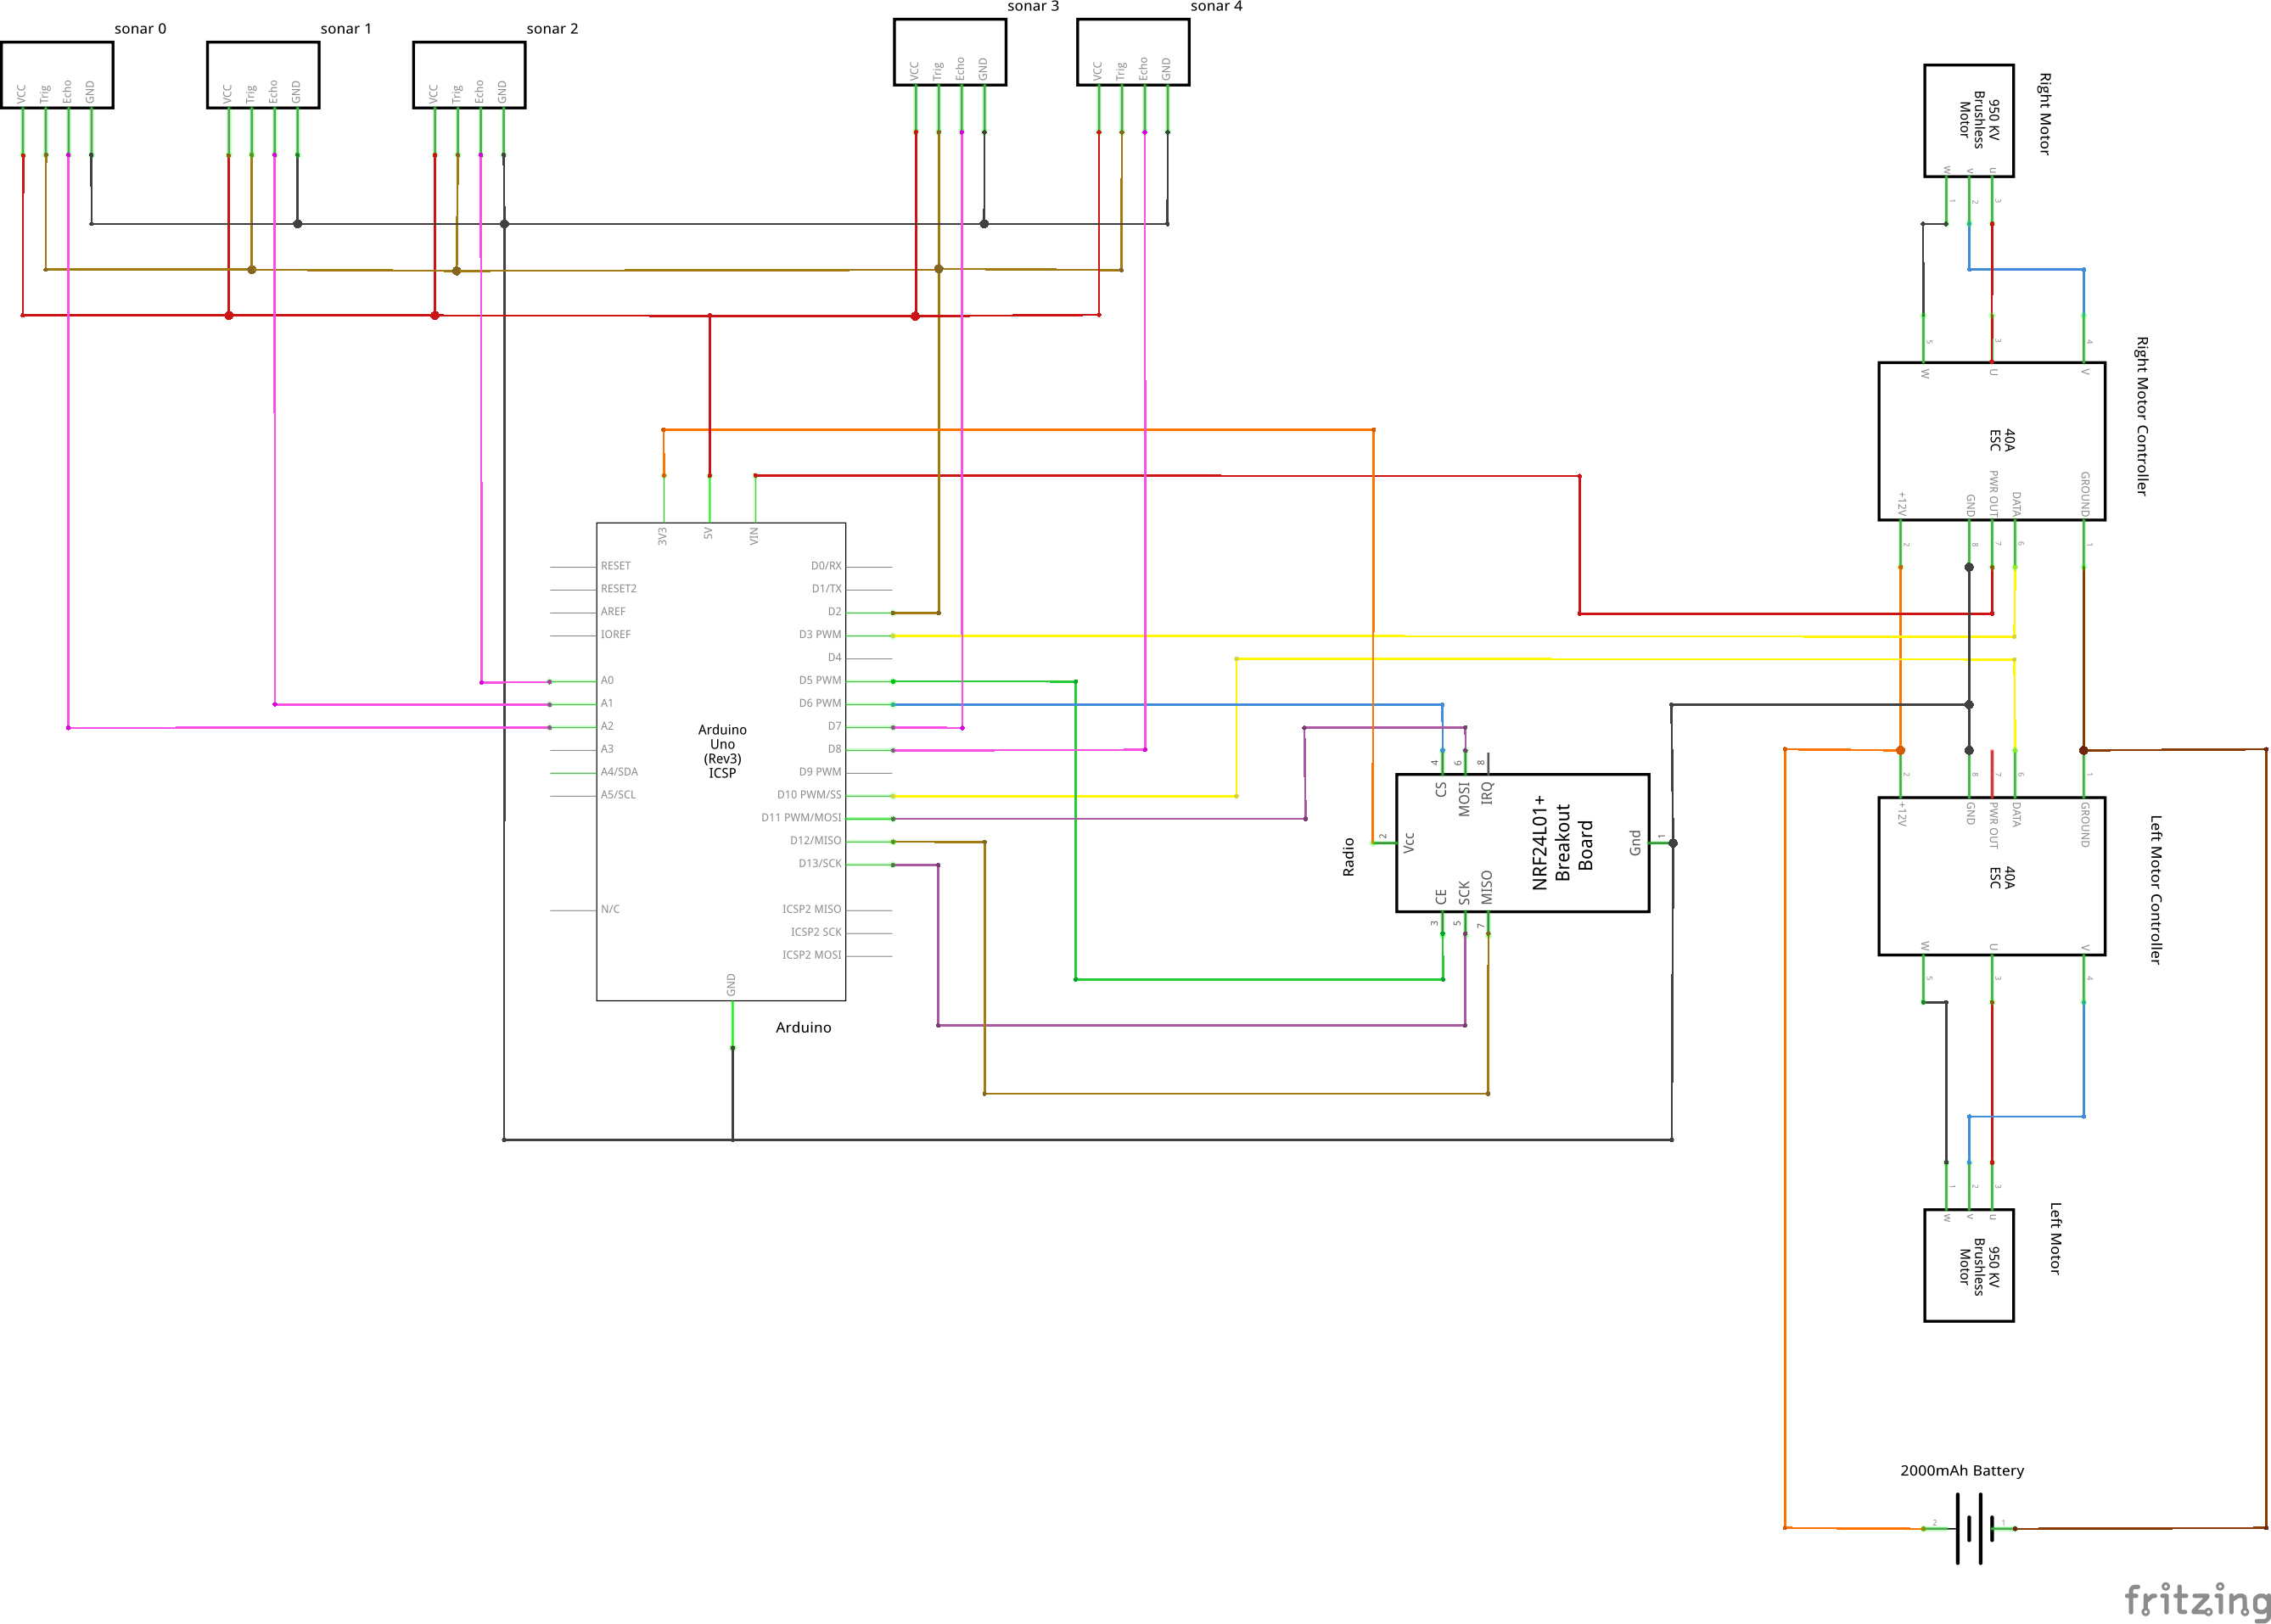
\includegraphics[width=\linewidth]{../../Imagens/robot_schem.png}
    \caption{Diagrama Elétrico} %% TODO: é um bom nome??
    \label{fritzing}
  \end{figure}
  
% TODO desatualizada!!!!
\section{Tabelas} % TODO desatualizada!!!!
% TODO desatualizada!!!!
\subsection{Tabela Verdade}
\begin{table}[!htb]
\centering
\caption{}
\label{IA}
\begin{tabular}{|ccccc|c|}
\hline
{\color[HTML]{00009B} \textbf{$USS_0$}} & {\color[HTML]{00009B} \textbf{$USS_1$}} & {\color[HTML]{00009B} \textbf{$USS_2$}} & 
{\color[HTML]{00009B} \textbf{$USS_3$}} & {\color[HTML]{00009B} \textbf{$USS_4$}} & {\color[HTML]{FE0000} \textbf{Ação}} \\ 
\hline
{\color[HTML]{00009B} 0}                                     & {\color[HTML]{00009B} 0}                                    & {\color[HTML]{00009B} 0} 
 
                                  & {\color[HTML]{00009B} 0}                                    & {\color[HTML]{00009B} 1}                            
 
       & {\color[HTML]{FE0000} $E_L$}                                     \\ \hline
{\color[HTML]{00009B} 0}                                     & {\color[HTML]{00009B} 0}                                    & {\color[HTML]{00009B} 0} 
 
                                  & {\color[HTML]{00009B} 1}                                    & {\color[HTML]{00009B} 0}                            
 
       & {\color[HTML]{FE0000} $E_M$}                                     \\ \hline
{\color[HTML]{00009B} 0}                                     & {\color[HTML]{00009B} 0}                                    & {\color[HTML]{00009B} 0} 
 
                                  & {\color[HTML]{00009B} 1}                                    & {\color[HTML]{00009B} 1}                            
 
       & {\color[HTML]{FE0000} $E_M$}                                     \\ \hline
{\color[HTML]{00009B} 0}                                     & {\color[HTML]{00009B} 0}                                    & {\color[HTML]{00009B} 1} 
 
                                  & {\color[HTML]{00009B} 0}                                    & {\color[HTML]{00009B} 0}                            
 
       & {\color[HTML]{FE0000} $E_F$}                                     \\ \hline
{\color[HTML]{00009B} 0}                                     & {\color[HTML]{00009B} 0}                                    & {\color[HTML]{00009B} 1} 
 
                                  & {\color[HTML]{00009B} 0}                                    & {\color[HTML]{00009B} 1}                            
 
       & {\color[HTML]{FE0000} $E_F$}                                     \\ \hline
{\color[HTML]{00009B} 0}                                   & {\color[HTML]{00009B} 0}                                    & {\color[HTML]{00009B} 1}   
 
                                & {\color[HTML]{00009B} 1}                                    & {\color[HTML]{00009B} 0}                              
 
     & {\color[HTML]{FE0000} $E_F$}                                     \\ \hline
{\color[HTML]{00009B} 0}                                    & {\color[HTML]{00009B} 0}                                  & {\color[HTML]{00009B} 1}    
 
                               & {\color[HTML]{00009B} 1}                                    & {\color[HTML]{00009B} 1}                               
 
    & {\color[HTML]{FE0000} $E_F$}                                     \\ \hline
{\color[HTML]{00009B} 0}                                     & {\color[HTML]{00009B} 1}                                    & {\color[HTML]{00009B} 0} 
 
                                & {\color[HTML]{00009B} 0}                                    & {\color[HTML]{00009B} 0}                              
 
     & {\color[HTML]{FE0000} $D_M$}                                     \\ \hline
{\color[HTML]{00009B} 0}                                    & {\color[HTML]{00009B} 1}                                    & {\color[HTML]{00009B} 0}  
 
                                 & {\color[HTML]{00009B} 0}                                 & {\color[HTML]{00009B} 1}                                
 
   & {\color[HTML]{FE0000} $D_M$}                                     \\ \hline
{\color[HTML]{00009B} 0}                                    & {\color[HTML]{00009B} 1}                                    & {\color[HTML]{00009B} 0}  
 
                                 & {\color[HTML]{00009B} 1}                                    & {\color[HTML]{00009B} 0}                             
 
      & {\color[HTML]{FE0000} $E_F$}                                     \\ \hline
{\color[HTML]{00009B} 0}                                    & {\color[HTML]{00009B} 1}                                    & {\color[HTML]{00009B} 0}  
 
                                 & {\color[HTML]{00009B} 1}                                    & {\color[HTML]{00009B} 1}                             
 
      & {\color[HTML]{FE0000} $E_M$}                                  \\ \hline
{\color[HTML]{00009B} 0}                                     & {\color[HTML]{00009B} 1}                                    & {\color[HTML]{00009B} 1} 
 
                                  & {\color[HTML]{00009B} 0}                                    & {\color[HTML]{00009B} 0}                            
 
       & {\color[HTML]{FE0000} $D_F$}                                     \\ \hline
{\color[HTML]{00009B} 0}                                     & {\color[HTML]{00009B} 1}                                    & {\color[HTML]{00009B} 1} 
 
                                  & {\color[HTML]{00009B} 0}                                    & {\color[HTML]{00009B} 1}                            
 
       & {\color[HTML]{FE0000} $E_F$}                                     \\ \hline
{\color[HTML]{00009B} 0}                                     & {\color[HTML]{00009B} 1}                                    & {\color[HTML]{00009B} 1} 
 
                                  & {\color[HTML]{00009B} 1}                                    & {\color[HTML]{00009B} 0}                            
 
       & {\color[HTML]{FE0000} $E_F$}                                     \\ \hline
{\color[HTML]{00009B} 0}                                     & {\color[HTML]{00009B} 1}                                    & {\color[HTML]{00009B} 1} 
 
                                  & {\color[HTML]{00009B} 1}                                    & {\color[HTML]{00009B} 1}                            
 
       & {\color[HTML]{FE0000} $E_F$}                                     \\ \hline
{\color[HTML]{00009B} 1}                                     & {\color[HTML]{00009B} 0}                                    & {\color[HTML]{00009B} 0} 
 
                                  & {\color[HTML]{00009B} 0}                                    & {\color[HTML]{00009B} 0}                            
 
       & {\color[HTML]{FE0000} $D_L$}                                     \\ \hline
{\color[HTML]{00009B} 1}                                     & {\color[HTML]{00009B} 0}                                    & {\color[HTML]{00009B} 0} 
 
                                  & {\color[HTML]{00009B} 0}                                    & {\color[HTML]{00009B} 1}                            
 
       & {\color[HTML]{FE0000} Frente}                                     \\ \hline
{\color[HTML]{00009B} 1}                                     & {\color[HTML]{00009B} 0}                                    & {\color[HTML]{00009B} 0} 
 
                                  & {\color[HTML]{00009B} 1}                                    & {\color[HTML]{00009B} 0}                            
 
       & {\color[HTML]{FE0000} $E_M$}                                     \\ \hline
{\color[HTML]{00009B} 1}                                     & {\color[HTML]{00009B} 0}                                    & {\color[HTML]{00009B} 0} 
 
                                  & {\color[HTML]{00009B} 1}                                    & {\color[HTML]{00009B} 1}                            
 
       & {\color[HTML]{FE0000} $E_M$}                                     \\ \hline
{\color[HTML]{00009B} 1}                                     & {\color[HTML]{00009B} 0}                                    & {\color[HTML]{00009B} 1} 
 
                                  & {\color[HTML]{00009B} 0}                                    & {\color[HTML]{00009B} 0}                            
 
       & {\color[HTML]{FE0000} $D_F$}                                     \\ \hline
{\color[HTML]{00009B} 1}                                     & {\color[HTML]{00009B} 0}                                    & {\color[HTML]{00009B} 1} 
 
                                  & {\color[HTML]{00009B} 0}                                    & {\color[HTML]{00009B} 1}                            
 
       & {\color[HTML]{FE0000} $E_F$}                                     \\ \hline
{\color[HTML]{00009B} 1}                                     & {\color[HTML]{00009B} 0}                                    & {\color[HTML]{00009B} 1} 
 
                                  & {\color[HTML]{00009B} 1}                                    & {\color[HTML]{00009B} 0}                            
 
       & {\color[HTML]{FE0000} $E_F$}                                     \\ \hline
{\color[HTML]{00009B} 1}                                     & {\color[HTML]{00009B} 0}                                    & {\color[HTML]{00009B} 1} 
 
                                  & {\color[HTML]{00009B} 1}                                    & {\color[HTML]{00009B} 1}                            
 
       & {\color[HTML]{FE0000} $E_F$}                                     \\ \hline
{\color[HTML]{00009B} 1}                                     & {\color[HTML]{00009B} 1}                                    & {\color[HTML]{00009B} 0} 
 
                                  & {\color[HTML]{00009B} 0}                                    & {\color[HTML]{00009B} 0}                            
 
       & {\color[HTML]{FE0000} $D_M$}                                     \\ \hline
{\color[HTML]{00009B} 1}                                     & {\color[HTML]{00009B} 1}                                    & {\color[HTML]{00009B} 0} 
 
                                  & {\color[HTML]{00009B} 0}                                    & {\color[HTML]{00009B} 1}                            
 
       & {\color[HTML]{FE0000} $D_M$}                                     \\ \hline
{\color[HTML]{00009B} 1}                                     & {\color[HTML]{00009B} 1}                                    & {\color[HTML]{00009B} 0} 
 
                                  & {\color[HTML]{00009B} 1}                                    & {\color[HTML]{00009B} 0}                            
 
       & {\color[HTML]{FE0000} $D_M$}                                     \\ \hline
{\color[HTML]{00009B} 1}                                     & {\color[HTML]{00009B} 1}                                    & {\color[HTML]{00009B} 0} 
 
                                  & {\color[HTML]{00009B} 1}                                    & {\color[HTML]{00009B} 1}                            
 
       & {\color[HTML]{FE0000} Frente}                                     \\ \hline
{\color[HTML]{00009B} 1}                                     & {\color[HTML]{00009B} 1}                                    & {\color[HTML]{00009B} 1} 
 
                                  & {\color[HTML]{00009B} 0}                                    & {\color[HTML]{00009B} 0}                            
 
       & {\color[HTML]{FE0000} $D_F$}                                     \\ \hline
{\color[HTML]{00009B} 1}                                     & {\color[HTML]{00009B} 1}                                    & {\color[HTML]{00009B} 1} 
 
                                  & {\color[HTML]{00009B} 0}                                    & {\color[HTML]{00009B} 1}                            
 
       & {\color[HTML]{FE0000} $D_F$}                                     \\ \hline
{\color[HTML]{00009B} 1}                                     & {\color[HTML]{00009B} 1}                                    & {\color[HTML]{00009B} 1} 
 
                                  & {\color[HTML]{00009B} 1}                                    & {\color[HTML]{00009B} 0}                            
 
       & {\color[HTML]{FE0000} $D_F$}                                     \\ \hline
{\color[HTML]{00009B} 1}                                     & {\color[HTML]{00009B} 1}                                    & {\color[HTML]{00009B} 1} 
 
                                  & {\color[HTML]{00009B} 1}                                    & {\color[HTML]{00009B} 1}                            
 
       & {\color[HTML]{FE0000} $E_F$}                                    \\ \hline

\end{tabular}
\end{table}



\subsection{Tabela Verdade para o Teste da Interferência dos BLDC nos Sonares}
\begin{table}[!htb]
\centering
\caption{My caption}
\label{tabela-interf}
\begin{tabular}{|ccccc|c|}
\hline
{\color[HTML]{00009B} $USS_0$} & {\color[HTML]{00009B} $USS_1$} & {\color[HTML]{00009B} $USS_2$} & {\color[HTML]{00009B} $USS_3$} & 
{\color[HTML]{00009B} $USS_4$} & {\color[HTML]{FE0000} \textbf{Ação}} \\ \hline
{\color[HTML]{00009B} 0}      & {\color[HTML]{00009B} X}      & {\color[HTML]{00009B} 0}      & {\color[HTML]{00009B} X}      & {\color[HTML]{00009B} 
0}      & {\color[HTML]{FE0000} $Frente$}             \\ \hline
{\color[HTML]{00009B} 0}      & {\color[HTML]{00009B} X}      & {\color[HTML]{00009B} 0}      & {\color[HTML]{00009B} X}      & {\color[HTML]{00009B} 
1}      & {\color[HTML]{FE0000} $E_F$}             \\ \hline
{\color[HTML]{00009B} 0}      & {\color[HTML]{00009B} X}      & {\color[HTML]{00009B} 1}      & {\color[HTML]{00009B} X}      & {\color[HTML]{00009B} 
0}      & {\color[HTML]{FE0000} $E_F$}             \\ \hline
{\color[HTML]{00009B} 0}      & {\color[HTML]{00009B} X}      & {\color[HTML]{00009B} 1}      & {\color[HTML]{00009B} X}      & {\color[HTML]{00009B} 
1}      & {\color[HTML]{FE0000} $E_F$}             \\ \hline
{\color[HTML]{00009B} 1}      & {\color[HTML]{00009B} X}      & {\color[HTML]{00009B} 0}      & {\color[HTML]{00009B} X}      & {\color[HTML]{00009B} 
0}      & {\color[HTML]{FE0000} $D_F$}             \\ \hline
{\color[HTML]{00009B} 1}      & {\color[HTML]{00009B} X}      & {\color[HTML]{00009B} 0}      & {\color[HTML]{00009B} X}      & {\color[HTML]{00009B} 
1}      & {\color[HTML]{FE0000} $Frente$}             \\ \hline
{\color[HTML]{00009B} 1}      & {\color[HTML]{00009B} X}      & {\color[HTML]{00009B} 1}      & {\color[HTML]{00009B} X}      & {\color[HTML]{00009B} 
0}      & {\color[HTML]{FE0000} $D_F$}             \\ \hline
{\color[HTML]{00009B} 1}      & {\color[HTML]{00009B} X}      & {\color[HTML]{00009B} 1}      & {\color[HTML]{00009B} X}      & {\color[HTML]{00009B} 
1}      & {\color[HTML]{FE0000} $E_F$}             \\ \hline
\end{tabular}
\end{table}


\section{Fluxograma da Rotina de Desvio de Obstáculos}
  \begin{figure}[!htb]
    \centering
    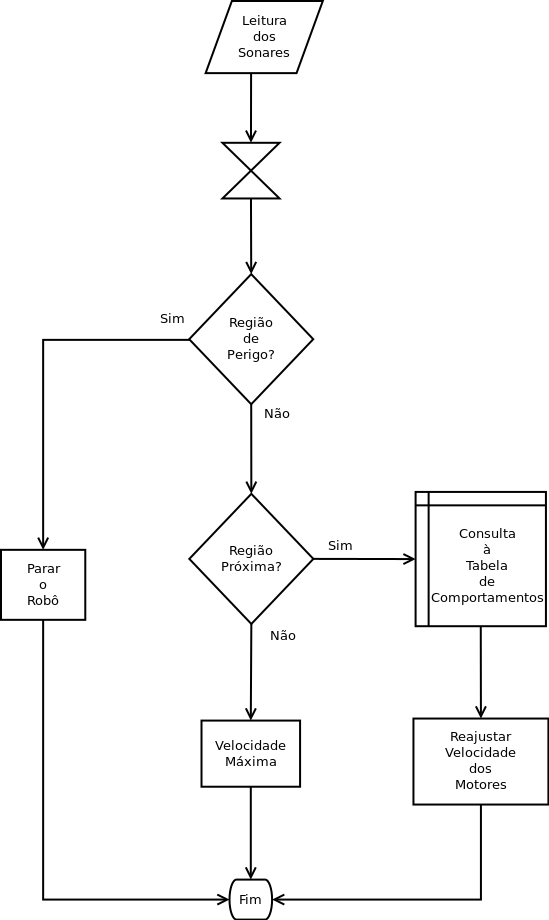
\includegraphics[width=0.8 \linewidth]{../../Imagens/ObstAvoid.png}
    \caption{Fluxograma da Rotina de Desvio de Obstáculos}
    \label{ObstAvoid}
  \end{figure}

\section{Sistemas de Tempo Real}
São sistemas computacionais que dependem não somente que os dados computados estejam corretos, mas que sejam obtidos dentro de um intervalo de tempo 
pré determinado, que pode ser maior ou menor de acordo com a aplicação.
Na literatura, este período em que se espera que a resposta do sistema se dê é denominado \textit{deadline}.
Sistemas de tempo real podem ser classificados em dois tipos: \textit{soft} ou \textit{hard}.

Sistemas \textit{soft} são menos restritivos, tolerando eventuais perdas de \textit{deadline}; 
ao contrário dos sistemas \textit{hard}, em que estas perdas não são aceitáveis.  

Algumas características típicas, apesar de não obrigatórias, de sistemas de tempo real são limitações com relação ao tamanho, propósito específico e 
baixo custo \cite{silberschatz}.

\section{CRC}
Método de detecção de erros aleatórios, isto é, de dados corrompidos ao longo do processo de transmissão ou armazenamento da informação por exemplo 
por ruídos, mas não por um agente \textquoteleft inteligente\textquoteright{} externo que modifique os dados transmitidos, tal qual um 
\textit{malware} \cite{stigge}.

Consiste essencialmente em uma divisão polinomial \cite{stigge}, logo, pode ser implementado em \textit{hardware}, utilizando-se apenas registradores 
de deslocamento com conexões realimentadas \cite{peterson}, assim como em \textit{software}. 
Em suma, trata-se de acrescentar à mensagem digital original um sufixo, que tem seu valor definido por operações realizadas em função da mensagem 
binária que intenta-se enviar e de um polinômio gerador.
Para o \textit{transceiver} nRF24L01+, dois polinômios geradores são utilizados: Eq. \ref{CRC_1} quando o dado cíclico adicionado é de 1 
\textit{byte} , e Eq. \ref{CRC_2}, para 2 \textit{bytes} \cite{nRF}.

Para uma descrição completa de como é implementado este método, vide \cite{stigge,peterson}.

\begin{equation}
\label{CRC_1}
G(X) = X^8 + X^2 + X + 1 
\end{equation}

\begin{equation}
\label{CRC_2}
G(X) = X^{16} + X^{12} + X^5 + 1 
\end{equation}

\section{MIFA} %% se der tempo, né?

\section{efeito hall} %% se der tempo, né?

\section{campo girante}

\section{\textit{schmitt trigger}}

\section{PWM}
A modulação por largura de pulso é uma técnica de modulação que consiste em amostrar e codificar o sinal correspondente à mensagem na largura de um 
trem de pulsos de amplitude fixa, i.e. cada amostra da mensagem é convertida em um pulso retangular cuja duração expressa a amplitude do sinal 
modulante.

Um modulador PWM pode ser implementado utilizando-se um circuito comparador não inversor cuja entrada inversora liga-se à saída de um gerador de 
ondas tipo dente de serra (\textit{trailing edge modulation}), dente de serra invertida (\textit{leading edge modulation}  ou triangular 
(\textit{modulation on both edges}), na entrada não inversora, o sinal modulante. 
Desta forma, quando a tensão da mensagem excede a amplitude da onda gerada, observa-se um sinal alto na saída, caso contrário, baixo, conforme 
ilustra a Fig. \ref{pwm_modulation_types}.

  \begin{figure}[!htb] %% TODO fonte: https://en.wikipedia.org/wiki/File:Three_PWM_types.svg
    \centering
    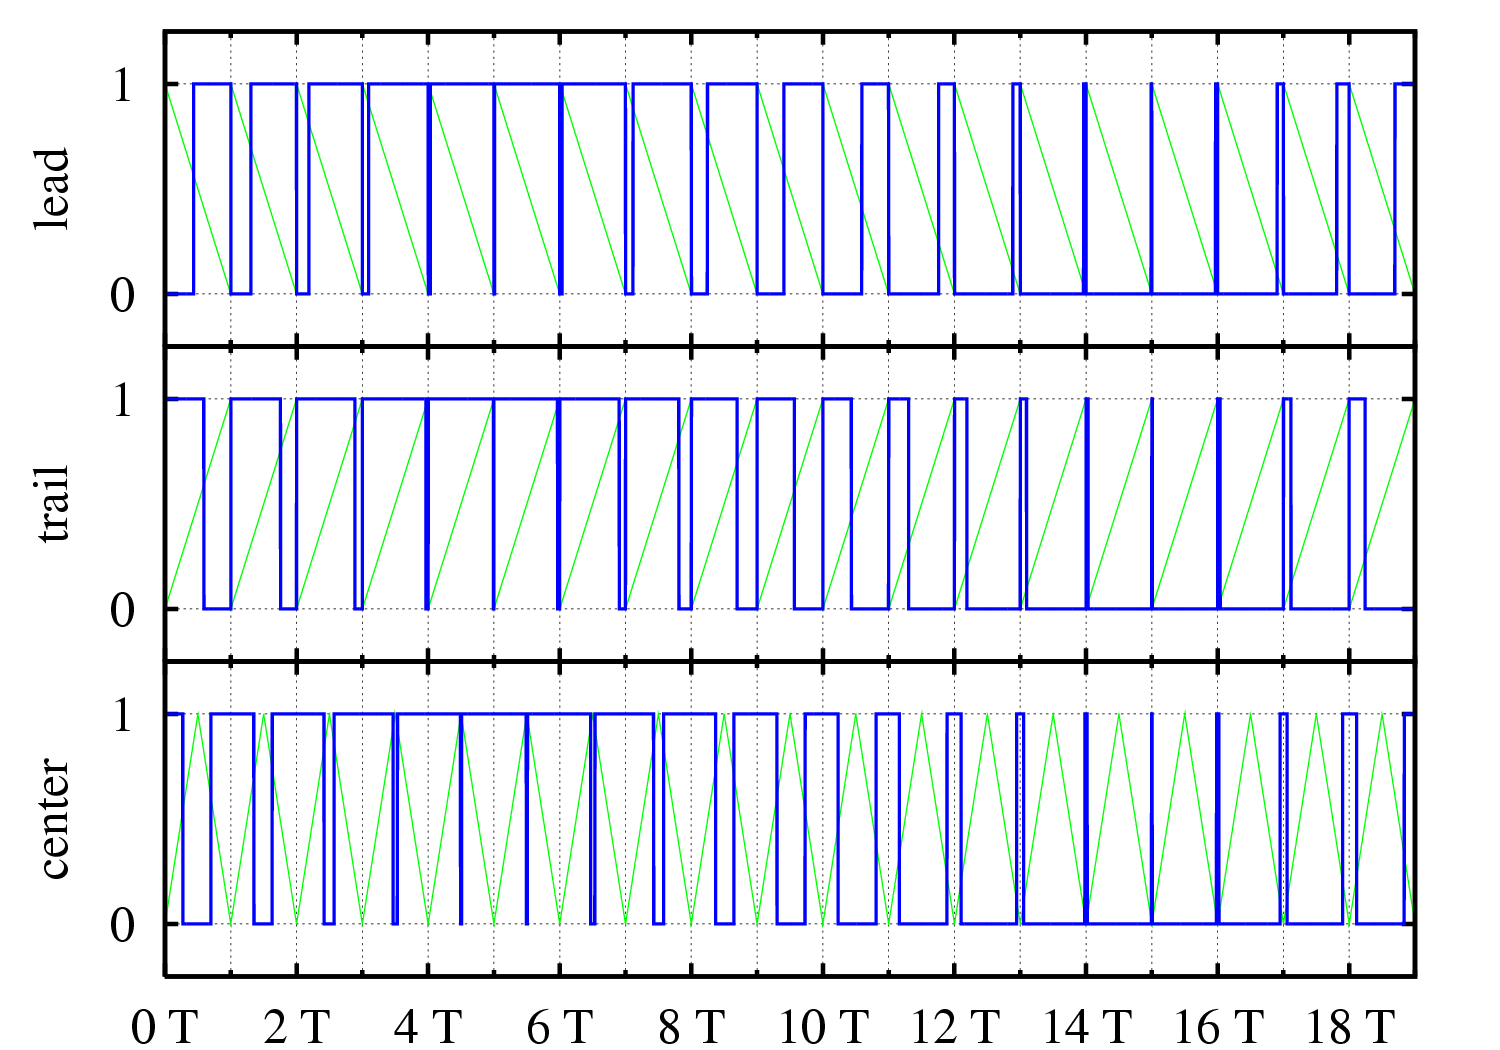
\includegraphics[width=0.7\linewidth]{../../Imagens/PWM_modulation_types.png}
    \caption{Três tipos de modulação PWM: \textit{trailing edge}, \textit{leading edge} e  \textit{both edges}, de cima pra baixo, respectivamente.}
    \label{pwm_modulation_types}
  \end{figure}
  
  %TODO circuito corretor de erros:
   First, the error amplifier accommodates feedback of the output PWM waveform in order to correct for any errors in the
output voltage introduced by the comparator. Second, it adds a dc offset to the input voltage so that negative input voltages can be accommodated by 
the circuit.
 
 Because the supply voltage of the comparator directly impacts the output voltage, PWM circuits without feedback have no power supply rejection. In 
this TI Design, the error amplifier acts as an inverting amplifier to the input signal, shown as a dc-coupled source VIN. By including the comparator 
inside the feedback loop of the error amplifier, and adding integration capacitor C1, the error amplifier now directly controls the average output 
voltage



para uma descrição detalhada do circuito e simulações vide \cite{pwm_modulator}

\section{GFSK}

\section{banda ISM}

\section{SPI}

\section{Testes Realizados}
\subsection{Interferência dos BLDC nos sonares}
\begin{table}[]
\centering
\caption{My caption}
\label{my-label}
\begin{tabular}{lllll|l|}
\hline
\multicolumn{1}{|c|}{\textbf{USS4}} & \multicolumn{1}{c|}{\textbf{USS3}} & \multicolumn{1}{c|}{\textbf{USS2}} & \multicolumn{1}{c|}{\textbf{USS1}} & 
\multicolumn{1}{c|}{\textbf{USS0}} & \multicolumn{1}{c|}{\textbf{Manobra}} \\ \hline
\multicolumn{1}{c}{273}             & \multicolumn{1}{c}{400}            & \multicolumn{1}{c}{400}            & \multicolumn{1}{c}{82}             & 
400                                & DF                                    \\ \hline
\multicolumn{1}{c}{211}             & \multicolumn{1}{c}{400}            & \multicolumn{1}{c}{400}            & \multicolumn{1}{c}{188}            & 
400                                & DF                                    \\ \hline
161                                 & 400                                & 400                                & 294                                & 
400                                & DF                                    \\ \hline
112                                 & 400                                & 400                                & 400                                & 
400                                & DF                                    \\ \hline
111                                 & 400                                & 400                                & 400                                & 
400                                & DF                                    \\ \hline
112                                 & 400                                & 400                                & 400                                & 
400                                & DF                                    \\ \hline
113                                 & 400                                & 400                                & 400                                & 
400                                & DF                                    \\ \hline
112                                 & 400                                & 400                                & 400                                & 
400                                & DF                                    \\ \hline
111                                 & 400                                & 400                                & 400                                & 
400                                & DF                                    \\ \hline
112                                 & 400                                & 400                                & 400                                & 
400                                & DF                                    \\ \hline
111                                 & 400                                & 400                                & 400                                & 
400                                & DF                                    \\ \hline
112                                 & 400                                & 400                                & 400                                & 
400                                & DF                                    \\ \hline
111                                 & 400                                & 400                                & 400                                & 
400                                & DF                                    \\ \hline
112                                 & 400                                & 400                                & 400                                & 
400                                & DF                                    \\ \hline
113                                 & 400                                & 400                                & 400                                & 
400                                & DF                                    \\ \hline
112                                 & 400                                & 400                                & 400                                & 
400                                & DF                                    \\ \hline
113                                 & 400                                & 400                                & 400                                & 
400                                & DF                                    \\ \hline
112                                 & 400                                & 400                                & 400                                & 
400                                & DF                                    \\ \hline
113                                 & 400                                & 400                                & 400                                & 
400                                & DF                                    \\ \hline
112                                 & 400                                & 400                                & 400                                & 
400                                & DF                                    \\ \hline
111                                 & 400                                & 400                                & 400                                & 
400                                & DF                                    \\ \hline
110                                 & 400                                & 400                                & 400                                & 
400                                & DF                                    \\ \hline
111                                 & 400                                & 400                                & 400                                & 
400                                & DF                                    \\ \hline
112                                 & 400                                & 400                                & 400                                & 
400                                & DF                                    \\ \hline
113                                 & 400                                & 400                                & 400                                & 
400                                & DF                                    \\ \hline
113                                 & 400                                & 400                                & 400                                & 
303                                & FS                                    \\ \hline
113                                 & 400                                & 400                                & 400                                & 
205                                & FS                                    \\ \hline
208                                 & 400                                & 400                                & 400                                & 
205                                & FS                                    \\ \hline
304                                 & 400                                & 400                                & 400                                & 
302                                & FS                                    \\ \hline
400                                 & 400                                & 400                                & 400                                & 
303                                & EF                                    \\ \hline
400                                 & 400                                & 400                                & 400                                & 
207                                & EF                                    \\ \hline
400                                 & 400                                & 400                                & 400                                & 
110                                & EF                                    \\ \hline
400                                 & 400                                & 400                                & 400                                & 
109                                & EF                                    \\ \hline
400                                 & 400                                & 400                                & 400                                & 
207                                & EF                                    \\ \hline
400                                 & 400                                & 400                                & 400                                & 
208                                & EF                                    \\ \hline
400                                 & 400                                & 400                                & 400                                & 
304                                & EF                                    \\ \hline
400                                 & 400                                & 400                                & 400                                & 
400                                & OR                                    \\ \hline
400                                 & 400                                & 400                                & 400                                & 
304                                & EF                                    \\ \hline
400                                 & 400                                & 400                                & 400                                & 
209                                & EF                                    \\ \hline
400                                 & 400                                & 400                                & 400                                & 
114                                & EF                                    \\ \hline
400                                 & 400                                & 400                                & 400                                & 
113                                & EF                                    \\ \hline
400                                 & 400                                & 400                                & 400                                & 
114                                & EF                                    \\ \hline
400                                 & 400                                & 400                                & 400                                & 
113                                & EF                                    \\ \hline
400                                 & 400                                & 400                                & 400                                & 
114                                & EF                                    \\ \hline
400                                 & 400                                & 400                                & 400                                & 
115                                & EF                                    \\ \hline
400                                 & 400                                & 400                                & 400                                & 
114                                & EF                                    \\ \hline
400                                 & 400                                & 400                                & 400                                & 
115                                & EF                                    \\ \hline
400                                 & 400                                & 400                                & 400                                & 
114                                & EF                                    \\ \hline
400                                 & 400                                & 400                                & 400                                & 
115                                & EF                                    \\ \hline
400                                 & 400                                & 400                                & 400                                & 
114                                & EF                                    \\ \hline
400                                 & 400                                & 400                                & 400                                & 
115                                & EF                                    \\ \hline
400                                 & 400                                & 400                                & 400                                & 
116                                & EF                                    \\ \hline
400                                 & 400                                & 400                                & 400                                & 
211                                & EF                                    \\ \hline
400                                 & 400                                & 400                                & 400                                & 
305                                & EF                                    \\ \hline
400                                 & 400                                & 400                                & 400                                & 
400                                & OR                                    \\ \hline
301                                 & 400                                & 400                                & 400                                & 
400                                & DF                                    \\ \hline
201                                 & 400                                & 400                                & 400                                & 
400                                & DF                                    \\ \hline
100                                 & 400                                & 400                                & 400                                & 
400                                & DF                                    \\ \hline
98                                  & 400                                & 400                                & 400                                & 
400                                & DF                                    \\ \hline
96                                  & 400                                & 400                                & 400                                & 
400                                & DF                                    \\ \hline
95                                  & 400                                & 400                                & 400                                & 
400                                & DF                                    \\ \hline
94                                  & 400                                & 400                                & 400                                & 
400                                & DF                                    \\ \hline
93                                  & 400                                & 400                                & 400                                & 
400                                & DF                                    \\ \hline
94                                  & 400                                & 400                                & 400                                & 
400                                & DF                                    \\ \hline
95                                  & 400                                & 400                                & 400                                & 
400                                & DF                                    \\ \hline
94                                  & 400                                & 400                                & 400                                & 
400                                & DF                                    \\ \hline
93                                  & 400                                & 400                                & 400                                & 
400                                & DF                                    \\ \hline
94                                  & 400                                & 400                                & 400                                & 
400                                & DF                                    \\ \hline
93                                  & 400                                & 400                                & 400                                & 
400                                & DF                                    \\ \hline
94                                  & 400                                & 400                                & 400                                & 
400                                & DF                                    \\ \hline
95                                  & 400                                & 400                                & 400                                & 
400                                & DF                                    \\ \hline
94                                  & 400                                & 400                                & 400                                & 
400                                & DF                                    \\ \hline
95                                  & 400                                & 400                                & 400                                & 
400                                & DF                                    \\ \hline
94                                  & 400                                & 400                                & 400                                & 
400                                & DF                                    \\ \hline
95                                  & 400                                & 400                                & 400                                & 
400                                & DF                                    \\ \hline
94                                  & 400                                & 400                                & 400                                & 
400                                & DF                                    \\ \hline
93                                  & 400                                & 400                                & 400                                & 
400                                & DF                                    \\ \hline
94                                  & 400                                & 400                                & 400                                & 
400                                & DF                                    \\ \hline
95                                  & 400                                & 400                                & 400                                & 
400                                & DF                                    \\ \hline
96                                  & 400                                & 400                                & 400                                & 
400                                & DF                                    \\ \hline
97                                  & 400                                & 400                                & 400                                & 
400                                & DF                                    \\ \hline
99                                  & 400                                & 400                                & 400                                & 
400                                & DF                                    \\ \hline
100                                 & 400                                & 400                                & 400                                & 
400                                & DF                                    \\ \hline
103                                 & 400                                & 400                                & 400                                & 
400                                & DF                                    \\ \hline
202                                 & 400                                & 400                                & 400                                & 
400                                & DF                                    \\ \hline
302                                 & 400                                & 400                                & 400                                & 
400                                & DF                                    \\ \hline
400                                 & 400                                & 400                                & 400                                & 
400                                & OR                                    \\ \hline
400                                 & 400                                & 400                                & 400                                & 
303                                & EF                                    \\ \hline
400                                 & 400                                & 400                                & 400                                & 
206                                & EF                                    \\ \hline
400                                 & 400                                & 400                                & 400                                & 
108                                & EF                                    \\ \hline
400                                 & 400                                & 400                                & 400                                & 
106                                & EF                                    \\ \hline
400                                 & 400                                & 400                                & 400                                & 
105                                & EF                                    \\ \hline
400                                 & 400                                & 400                                & 400                                & 
104                                & EF                                    \\ \hline
400                                 & 400                                & 400                                & 365                                & 
104                                & EF                                    \\ \hline
400                                 & 400                                & 400                                & 267                                & 
103                                & EF                                    \\ \hline
400                                 & 400                                & 400                                & 267                                & 
101                                & EF                                    \\ \hline
400                                 & 400                                & 400                                & 169                                & 
100                                & EF                                    \\ \hline
400                                 & 400                                & 400                                & 106                                & 
99                                 & EF                                    \\ \hline
400                                 & 400                                & 400                                & 105                                & 
99                                 & EF                                    \\ \hline
400                                 & 400                                & 400                                & 105                                & 
100                                & EF                                    \\ \hline
400                                 & 400                                & 400                                & 105                                & 
101                                & EF                                    \\ \hline
400                                 & 400                                & 400                                & 105                                & 
100                                & EF                                    \\ \hline
400                                 & 400                                & 400                                & 105                                & 
99                                 & EF                                    \\ \hline
400                                 & 400                                & 400                                & 105                                & 
98                                 & EF                                    \\ \hline
400                                 & 400                                & 400                                & 104                                & 
97                                 & EF                                    \\ \hline
400                                 & 400                                & 400                                & 104                                & 
80                                 & EF                                    \\ \hline
400                                 & 400                                & 400                                & 104                                & 
64                                 & EF                                    \\ \hline
400                                 & 400                                & 400                                & 104                                & 
48                                 & STP                                   \\ \hline
400                                 & 400                                & 400                                & 104                                & 
49                                 & STP                                   \\ \hline
400                                 & 400                                & 400                                & 105                                & 
49                                 & STP                                   \\ \hline
400                                 & 400                                & 400                                & 104                                & 
49                                 & STP                                   \\ \hline
400                                 & 400                                & 400                                & 105                                & 
49                                 & STP                                   \\ \hline
400                                 & 400                                & 400                                & 105                                & 
65                                 & EF                                    \\ \hline
400                                 & 400                                & 400                                & 105                                & 
82                                 & EF                                    \\ \hline
400                                 & 400                                & 400                                & 105                                & 
97                                 & EF                                    \\ \hline
400                                 & 400                                & 400                                & 105                                & 
98                                 & EF                                    \\ \hline
400                                 & 400                                & 400                                & 106                                & 
98                                 & EF                                    \\ \hline
400                                 & 400                                & 400                                & 204                                & 
100                                & EF                                    \\ \hline
400                                 & 400                                & 400                                & 302                                & 
102                                & EF                                    \\ \hline
400                                 & 400                                & 400                                & 400                                & 
105                                & EF                                    \\ \hline
400                                 & 400                                & 400                                & 400                                & 
108                                & EF                                    \\ \hline
400                                 & 400                                & 400                                & 400                                & 
110                                & EF                                    \\ \hline
400                                 & 400                                & 400                                & 400                                & 
112                                & EF                                    \\ \hline
400                                 & 400                                & 400                                & 400                                & 
114                                & EF                                    \\ \hline
400                                 & 400                                & 400                                & 400                                & 
115                                & EF                                    \\ \hline
400                                 & 400                                & 400                                & 400                                & 
114                                & EF                                    \\ \hline
400                                 & 400                                & 400                                & 400                                & 
113                                & EF                                    \\ \hline
400                                 & 400                                & 400                                & 400                                & 
112                                & EF                                    \\ \hline
400                                 & 400                                & 400                                & 400                                & 
113                                & EF                                    \\ \hline
400                                 & 400                                & 400                                & 400                                & 
210                                & EF                                    \\ \hline
400                                 & 400                                & 400                                & 400                                & 
305                                & EF                                    \\ \hline
400                                 & 400                                & 400                                & 400                                & 
400                                & OR                                    \\ \hline
303                                 & 400                                & 400                                & 400                                & 
400                                & DF                                    \\ \hline
205                                 & 400                                & 400                                & 400                                & 
400                                & DF                                    \\ \hline
303                                 & 400                                & 400                                & 400                                & 
400                                & DF                                    \\ \hline
400                                 & 400                                & 400                                & 400                                & 
400                                & OR                                    \\ \hline
302                                 & 400                                & 400                                & 400                                & 
400                                & DF                                    \\ \hline
203                                 & 400                                & 400                                & 400                                & 
400                                & DF                                    \\ \hline
104                                 & 400                                & 400                                & 400                                & 
400                                & DF                                    \\ \hline
103                                 & 400                                & 400                                & 400                                & 
400                                & DF                                    \\ \hline
85                                  & 400                                & 400                                & 400                                & 
400                                & DF                                    \\ \hline
66                                  & 400                                & 400                                & 400                                & 
400                                & DF                                    \\ \hline
47                                  & 400                                & 400                                & 400                                & 
400                                & STP                                   \\ \hline
39                                  & 400                                & 400                                & 400                                & 
400                                & STP                                   \\ \hline
49                                  & 400                                & 400                                & 400                                & 
400                                & STP                                   \\ \hline
31                                  & 400                                & 400                                & 400                                & 
400                                & STP                                   \\ \hline
42                                  & 400                                & 400                                & 400                                & 
400                                & STP                                   \\ \hline
58                                  & 400                                & 400                                & 400                                & 
400                                & DF                                    \\ \hline
73                                  & 400                                & 400                                & 400                                & 
400                                & DF                                    \\ \hline
74                                  & 400                                & 400                                & 400                                & 
400                                & DF                                    \\ \hline
75                                  & 400                                & 400                                & 400                                & 
400                                & DF                                    \\ \hline
81                                  & 400                                & 400                                & 400                                & 
400                                & DF                                    \\ \hline
86                                  & 400                                & 400                                & 400                                & 
400                                & DF                                    \\ \hline
90                                  & 400                                & 400                                & 400                                & 
400                                & DF                                    \\ \hline
90                                  & 400                                & 400                                & 278                                & 
400                                & DF                                    \\ \hline
90                                  & 400                                & 400                                & 156                                & 
400                                & DF                                    \\ \hline
93                                  & 400                                & 400                                & 39                                 & 
400                                & DF                                    \\ \hline
94                                  & 400                                & 400                                & 37                                 & 
400                                & DF                                    \\ \hline
97                                  & 400                                & 400                                & 43                                 & 
400                                & DF                                    \\ \hline
100                                 & 400                                & 400                                & 49                                 & 
400                                & DF                                    \\ \hline
101                                 & 400                                & 400                                & 51                                 & 
400                                & DF                                    \\ \hline
101                                 & 400                                & 400                                & 56                                 & 
400                                & DF                                    \\ \hline
101                                 & 400                                & 400                                & 60                                 & 
400                                & DF                                    \\ \hline
105                                 & 400                                & 400                                & 63                                 & 
400                                & DF                                    \\ \hline
108                                 & 400                                & 400                                & 70                                 & 
400                                & DF                                    \\ \hline
193                                 & 400                                & 400                                & 74                                 & 
400                                & DF                                    \\ \hline
290                                 & 400                                & 400                                & 74                                 & 
400                                & DF                                    \\ \hline
385                                 & 400                                & 400                                & 78                                 & 
400                                & OR                                    \\ \hline
400                                 & 400                                & 400                                & 79                                 & 
400                                & OR                                    \\ \hline
393                                 & 400                                & 400                                & 80                                 & 
400                                & OR                                    \\ \hline
387                                 & 400                                & 400                                & 81                                 & 
400                                & OR                                    \\ \hline
379                                 & 400                                & 400                                & 82                                 & 
400                                & OR                                    \\ \hline
377                                 & 400                                & 400                                & 83                                 & 
400                                & OR                                    \\ \hline
374                                 & 400                                & 400                                & 84                                 & 
400                                & OR                                    \\ \hline
                                    &                                    &                                    &                                    &   
                                 &                                       \\ \hline
\end{tabular}
\end{table}